\documentclass[runningheads]{llncs}
\usepackage{graphicx}
\usepackage[text={150mm,220mm},centering,nohead]{geometry}
\usepackage{float}
\pagestyle{empty} 
\begin{document}
\title{\large{Service-Oriented Software Engineering (Project Proposal)}}
\author{}
\institute{}
\maketitle
\vspace{-1cm}
%-----------Please Do NOT change the content above.-----------------

%---------------------------------------------------------------------------------------------------------------------------------

%-----------Please write the project information here.---------------

\begin{center}
\Large{\textbf{Meeting-Room Booking System}} \\ % Please write your project tile in here
\vspace{0.2cm}
\large{\emph{Group Members (2): ZijiaHe, WangZhihuimei}} \\%Please write names of your group members as well as the group number in here
\vspace{0.3cm}  
\end{center}

%-----------Please write the content of your research proposal from here.---------------
\noindent
\section{Project Charter}
\textbf{Project Title:} Meeting-Room Booking System\\
\textbf{Date of Authorization:} March 1\\
\textbf{Project Start Date:} March 18\\
\textbf{Project Finish Date:} May 5\\
\textbf{Key Schedule Milestones:}\\(1)Preparations Completed by April 3\\(2)Demo Version completed by April 28\\(3)Officially released\\
\textbf{Budget Information:}The firm has allocated \textbf{RMB56800} for this project,and more funds are available if needed.The majority cost for this project will be internal labor.\\
\textbf{Project Manager:}\textbf{Wangzhihui Mei},your email; \textbf{Zijia He},296344774@qq.com\\
\textbf{Project Objectives:}Meeting-Room Booking System is a system that JI urgently needs. Our goal is to develop this system within two months\\
\textbf{Main Project Success Criteria:}The software can perfectly realize the functions of registering, logging in, booking classroom, unsubscribing classroom, and checking classroom status. At the same time, the entire project can be completed on schedule.\\
\textbf{Approach:}
(1)Planning the time in advance to ensure that the deadline can be completed as scheduled\\
(2)Determining the framework and technology used as early as possible.Drawing a Gantt chart to clarify the overall workflow and progress.\\\
(3)Holding a meeting once a week to ensure that the construction period is as usual
(4)Perform a series of tests for each new function\\
\begin{table}
\centering
\begin{tabular}{|c|c|c|}
\hline
\multicolumn{3}{|c|}{\textbf{ROLES AND RESPONSIBILITIES}}\\ % 用\multicolumn{3}表示横向合并三列 
                        % |c|表示居中并且单元格两侧添加竖线 最后是文本
\hline
\textbf{Name}&\textbf{Role}&\textbf{Contact Information}\\
\hline
Zijia He&Test engineer,Front-end engineer& 296344774@qq.com\\
\hline
Wangzhihui Mei&Project Manager,Front-end engineer,Backend engineer&Your@email.com\\
\hline
\end{tabular}
\end{table}



\section{Project Plans}
\subsection{Project Scope Statement}
\textbf{Product scope description}\\
The software developed in this project is used to book classrooms for JI students.The main functions of this software are user registration, user login, book classroom, unsubscribe classroom, and view the current classroom status.When the user has no registered member, they can only browse the classroom status and cannot book the classroom.When a classroom is booked, the classroom can only be booked again unless the applicant unsubscribes from the classroom or exceeds the scheduled usage time. Otherwise, the classroom will show the status of reservation.\\\\
\textbf{Product user acceptance criteria}\\
\textbf{Target Dates:}The first version of this system should be completed by April 28 and the final version should be completed by May 5.\\
\textbf{Major function:}This system is divided into client and administrator.On the client side, the client can select the classroom, unsubscribe the classroom, and view the current status of the classroom.The administrator can view the user's reservation records and the current classroom status, and can force the user to unsubscribe.\\\\
\textbf{Detailed information on all project deliverables:}
1.Project Charter\\
2.Project Scope Statement\\
3.Project Schedule\\
4.Cost Management Plan\\
5.Human resource plan\\
6.Microsoft Project outputs for project schedule\\
7.Microsoft Project outputs for Cost Management\\
8.Microsoft Project outputs for Human resource allocation\\
9.Project progress report\\
10.Project closing and lessons-learnt\\
11.Meeting-Room Booking System\\
12.Tutorial of using Meeting-Room Booking System\\
\subsection{Project Schedule}
\begin{table}
\centering
\begin{tabular}{|c|c|c|c|c|}
\hline
\multicolumn{5}{|c|}{\textbf{Schedule}}\\ % 用\multicolumn{3}表示横向合并三列 
                        % |c|表示居中并且单元格两侧添加竖线 最后是文本
\hline
\textbf{Number}&\textbf{Task}&\textbf{Start Date}&\textbf{Finish Date}&\textbf{Participant}\\
\hline
1&Demand Analysis&18/3/2020&30/3/2020&Zijia He,Wangzhihui Mei\\
\hline
2&Architecture Design&23/3/2020&27/3/2020&Zijia He,Wangzhihui Mei\\
\hline
3&UI Design&30/3/2020&3/4/2020&Zijia He,Wangzhihui Mei\\
\hline
4&Server Development&6/4/2020&14/4/2020&Wangzhihui Mei\\
\hline
5&Unit Test&6/4/2020&14/4/2020&Zijia He\\
\hline
6&Front-End Development&6/4/2020&14/4/2020&Zijia He,Wangzhihui Mei\\
\hline
7&API Adaptation&15/4/2020&23/4/2020&Wangzhihui Mei\\
\hline
8&Bale&24/4/2020&27/4/2020&Wangzhihui Mei\\
\hline
9&Pressure Test&28/4/2020&28/4/2020&Zijia He\\
\hline
10&Integration Testing&29/4/2020&1/5/2020&Zijia He\\
\hline
11&Code Review&4/5/2020&5/5/2020&Wangzhihui Mei,Zijia He\\
\hline
\end{tabular}
\end{table}

\subsection{Cost Management Plan}
\textbf{Level of accuracy units of measure:} \textbf{RMB}\\
\textbf{Control Threshold:} \textbf{RMB100000}\\
\textbf{Rules of performance measurement:}\\
(1)Whether the staff completed the work on time\\
(2)The number of bugs in the test\\
\textbf{Budget:}\\
\textbf{Salary:}RMB56800\\
\textbf{Maintenance Cost:}RMB10000\\
\textbf{Image copyright:}RMB200
\subsection{Human resource plan}
\begin{figure}[H]
\centering
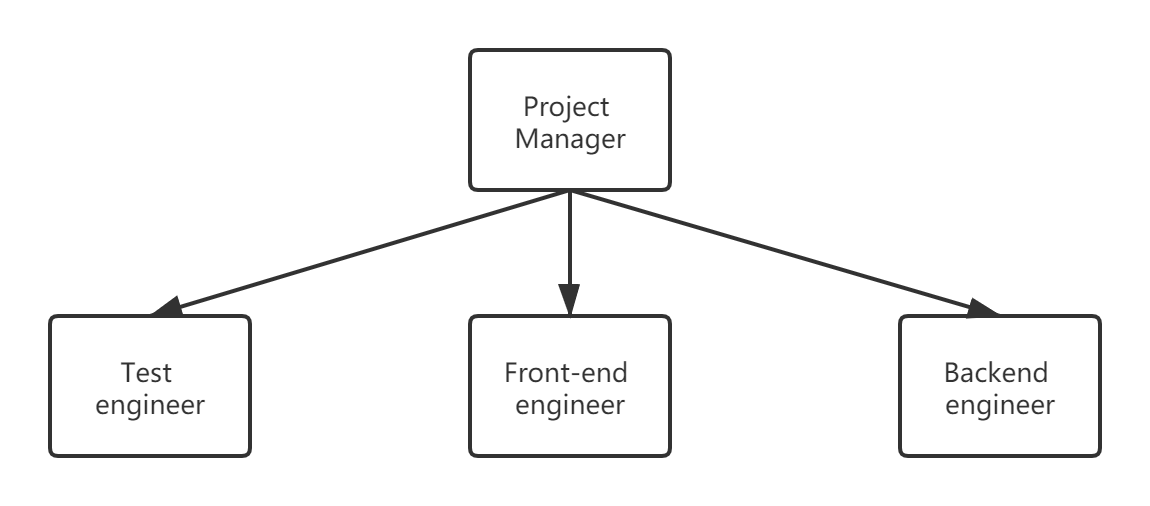
\includegraphics[width=4.5in]{1.png}
\end{figure}
\textbf{Staffing management plan:}\\
\textbf{Project Manager:}

Determine what kind of product to develop, what business model and business model to choose, etc. And promote the corresponding product development organization, he also needs to coordinate research and development, marketing, operation, etc. according to the product life cycle, determine and organize the implementation of the corresponding product strategy, and other related product management activities.\\
\textbf{Test engineer:}Test engineers should write test plans, plan detailed test plans, and write test cases. In addition, the test engineer needs to put forward suggestions for further product improvement and evaluate whether the improvement plan is reasonable; summarize and statistically analyze the test results, track the test, and provide feedback.\\
\textbf{Front-end engineer:}The front-end engineer is responsible for the layout design, page design and interaction design of the system ui.\\
\textbf{Backend engineer:}The back-end engineer is responsible for the background construction, database management, API management.
\begin{table}
\centering
\begin{tabular}{|c|c|c|c|c|}
\hline
\multicolumn{5}{|c|}{\textbf{Responsibility assignment matrixes}}\\ % 用\multicolumn{3}表示横向合并三列 
                        % |c|表示居中并且单元格两侧添加竖线 最后是文本
\hline
\textbf{Task}&\textbf{Project Manager}&\textbf{Test engineer}&\textbf{Front-end engineer}&\textbf{Backend engineer}\\
\hline
Demand Analysis&P,R&P&P&P\\
\hline
Architecture Design&P,R&P&P&P\\
\hline
UI Design&P&P&P,R&P\\
\hline
Server Development&N&N&N&P,R\\
\hline
Unit Test&N&R,P&N&N\\
\hline
Front-End Development&N&N&P,R&N\\
\hline
API Adaptation&N&N&N&P,R\\
\hline
Bale&N&N&N&P,R\\
\hline
Pressure Test&N&P,R&N&N\\
\hline
Integration Testing&N&P,R&N&N\\
\hline
Code Review&N&P&P&P,R\\
\hline

\end{tabular}
\caption{R:Responsibility  N:None  P:Participate}
\end{table}

\section{Project execution}
%Each team should provide sufficient details about how the project is executed. Thus, using the milestones you have identified in your project plan, you are required to demonstrate how your team has executed the project. For each milestone, you should update your project progress in terms of schedule and cost. For each milestone, appropriate project progress reports need to be generated and you should use Microsoft Project to track your project progress (appropriate baseline should be used to track the project progress). In addition to the outputs from Microsoft Project, you may also want to include the following in the report: project staff assignment, change requests, project management plan updates, deliverables, and at least 4 meeting minutes in the report.
There are 3 phase in out project: Product Design, Development and Release. Accordingly, There is a milestone in the end of each phase.


\subsection{Product Design}
The total cost of this phase is ¥20800 and 208 working hours. 

During This phase, out team performed Demand Analysis from Mar. 18 to May. 20 with the cost of ¥4800.
We finished the demand analysis within 48 hours, the baseline


\end{document}

